\documentclass[10pt,openright,twoside,french]{book}

\input philippe2013
\input philippe2013_cours
\input philippe2013_sections
\input philippe2013_chapitre

\pagestyle{empty}
\pieddepage{}{}{}

\setcounter{chapter}{5}
\begin{document}

\renewcommand\PartProgramme{Stats/Probas}
\chapter[Statistiques discrètes]{Statistiques descriptives discrètes\\ Analyse de données}\label{ch_statistiques_discretes}

\begin{Exemple}
On considère le relevé des températures en janvier et en février dans une ville :
\begin{center}
\renewcommand\arraystretch{1.5}
    \begin{tabular}{*{10}{|c}|}
        \hline
            \multicolumn{10}{|c|}{Janvier}\\
        \hline
            Valeurs & $-3\degres$ & $-2\degres$ & $-1\degres$ & $0\degres$ & $1\degres$ & $2\degres$ & $3\degres$ & $4\degres$ & Total \\
        \hline
            Effectifs & $3$ & $5$ & $8$ & $5$ & $4$ & $3$ & $2$ & $1$ & $31$\\
        \hline
            \multicolumn{10}{|c|}{Février}\\
        \hline
            Valeurs & $-3\degres$ & $-2\degres$ & $-1\degres$ & $0\degres$ & $1\degres$ & $2\degres$ & $3\degres$ & $4\degres$ & Total \\
        \hline
            Effectifs & $1$ & $2$ & $3$ & $3$ & $5$ & $9$ & $3$ & $2$ & $28$\\
            \hline
    \end{tabular}
\renewcommand\arraystretch{1}
\end{center}
\end{Exemple}

\section{L'étendue}
\begin{Defi}\index{etendue@étendue}
    Dans une série statistique, on appelle \iptb{étendue} la différence entre la plus grande valeur et la plus petite.
\end{Defi}

\begin{Exemple}
    Janvier :\par\bigskip
    Février :
\end{Exemple}


\section{Caractéristiques de position}
\subsection{Moyenne}

\begin{Defi}
    On considère une série statistique à valeurs numériques (série statistique quantitative). La \ipt{moyenne} $M$ de cette série se calcule de la façon suivante :
    \[\pfr{M = \dfrac{\text{somme des valeurs}}{\text{effectif total}}}\]
    Dans le cas où les valeurs ont des effectifs (ou c{\oe}fficients) supérieurs à 1, on utilise aussi :
    \[\pfr{M = \dfrac{\text{somme des (valeur $\times$ effectif)}}{\text{effectif total}}}\]
\end{Defi}


\begin{Exemple}

\end{Exemple}\clearpage

\subsection{Médiane}

\begin{Defi}
    On considère une série statistique dont l'effectif total est égal à $N$. Les valeurs sont rangées dans l'ordre croissant.

    \textbf{Une} \ipt{médiane} $Me$ est un nombre réel qui permet de partager la série statistique en deux séries de même valeur.

    Autrement dit, la moitié ($50\%$) des valeurs de la série est inférieure ou égale à $Me$ et l'autre moitié est supérieure ou égale à $Me$.

\begin{center}
    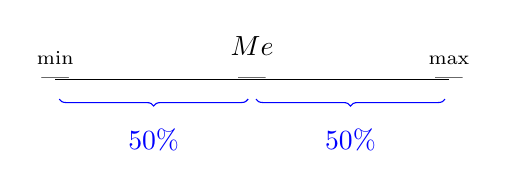
\begin{tikzpicture}
        \draw (0,0)--(5,0) node[midway] {|} node[midway,above=5pt] {$Me$};
        \draw (0,0) node {|} node[above=2pt] {\scriptsize $\min$}; \draw (5,0) node {|} node[above=2pt] {\scriptsize $\max$};
        \draw[color=blue,decorate,decoration={brace,raise=0.25cm}] (2.45,0) -- (0.05,0) node[below=0.5cm,pos=0.5] {$50\%$};
        \draw[color=blue,decorate,decoration={brace,raise=0.25cm}] (4.95,0) -- (2.55,0) node[below=0.5cm,pos=0.5] {$50\%$};
    \end{tikzpicture}
\end{center}
\end{Defi}

\textbf{Méthode de calcul :} Par définition, la médiane dépend de l'effectif de la série :
\begin{itemize}
    \item Si $N$ est impair, alors on calcule $\frac{N + 1}{2}$ et le résultat correspond à la position de la médiane choisie dans la série.
    \item Si $N$ est pair, alors la médiane choisie est égale à la moyenne de la valeur situé à la position $\frac N 2$ et la valeur suivante.
\end{itemize}

\begin{Exemple}

\end{Exemple}\vspace*{2cm}

\subsection{Quartiles}

\begin{Defi}
    On considère une série statistique $S$ dont l'effectif total est égal à $N$. Les valeurs sont rangées dans l'ordre croissant.
    \begin{itemize}
        \item Le \ipt{premier quartile}\index{quartile} $Q_1$ de $S$ est le plus petit élément $a$ de $S$ tel qu'au moins $25\%$ des données soient inférieures ou égales à $a$.
        \item Le \ipt{troisième quartile}\index{quartile} $Q_3$ de $S$ est le plus petit élément $b$ de $S$ tel qu'au moins $75\%$ des données soient inférieures ou égales à $b$.
    \end{itemize}

\begin{center}
    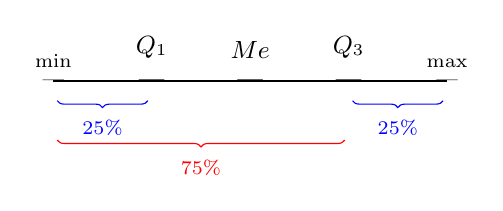
\begin{tikzpicture}
        \begin{small}
        \draw (0,0)--(5,0) node[midway] {|} node[midway,above=5pt] {$Me$} node[pos=0.75,above=5pt] {$Q_3$} node[pos=0.25,above=5pt] {$Q_1$};
        \draw (0,0)--(5,0) node[pos=0.25] {|}; \draw (0,0)--(5,0) node[pos=0.75] {|};
        \end{small}
        \begin{scriptsize}
        \draw (0,0) node {|} node[above=2pt] {$\min$}; \draw (5,0) node {|} node[above=2pt] {$\max$};
        \draw[color=blue,decorate,decoration={brace,raise=0.25cm}] (1.2,0) -- (0.05,0) node[below=0.4cm,pos=0.5] {$25\%$};
        \draw[color=blue,decorate,decoration={brace,raise=0.25cm}] (4.95,0) -- (3.8,0) node[below=0.4cm,pos=0.5] {$25\%$};
        \draw[color=red,decorate,decoration={brace,raise=0.75cm}] (3.7,0) -- (0.05,0) node[below=0.9cm,pos=0.5] {$75\%$};
        \end{scriptsize}
    \end{tikzpicture}
\end{center}
\end{Defi}

\textbf{Méthode de calcul :} Par définition, les quartiles dépendent de l'effectif de la série :
\begin{description}
    \item[Premier quartile :] On arrondit le nombre $\frac{N}{4}$ à l'unité par excès et cela donne la position de $Q_1$ dans la série $S$.
    \item[Troisième quartile :] On arrondit le nombre $3\times\frac{N}{4}$ à l'unité par excès et cela donne la position de $Q_3$ dans la série $S$.
\end{description}

\begin{Exemple}

\end{Exemple}

\end{document} 